Upravljački softver (eng. \textit{firmware}) kontrolira komponente i komunicira s aplikacijom prilikom autorizacije
kartice.
Napisan je u \textit{C++} programskom jeziku i \textit{Arduino} radnom okviru.
Kompiliranje izvornog koda i učitavanje binarnog koda u mikrokontroler omogućava \textit{PlatformIO}.

\subsection{Konfiguracija pinova i bežične mreže}

Prema schemi komponenti (slika~\ref{fig:component-schema}) definirane su vrijednosti pinova:

\begin{lstlisting}[language=C++]
#define RST_PIN     0
#define SS_PIN      5

#define LOCK_PIN    13
#define STATE_PIN   33

#define RED_PIN     27
#define GREEN_PIN   26
#define BLUE_PIN    25

#define ACCESS_POINT_NAME       "BoxAP"
#define ACCESS_POINT_PASSWORD   "********"
\end{lstlisting}

Potrebno je instancirati određene objekte:

\begin{lstlisting}[language=C++]
BoxAuthorizer authorizer = BoxAuthorizer();
Box box = Box(LOCK_PIN, STATE_PIN, authorizer);
CardReader reader = CardReader(SS_PIN, RST_PIN);
StatusLED LED = StatusLED(GREEN_PIN, RED_PIN, BLUE_PIN);
\end{lstlisting}

Mikrokontroler zahtjeva dvije funkcije u glavnom programu: \textbf{setup} i \textbf{loop}.
Funkcija \textit{setup} izvodi se samo jednom, pri paljenju mikrokontrolera.
Funkcija \textit{loop} izvršava se više puta (poput \textit{for} ili \textit{while} petlje) sve dok se mikrokontroler
ne ugasi.

Funkcija \textit{setup} je pogodna za inicijalnu pripremu i konfiguraciju pinova i povezivanje na bežičnu mrežu.

\begin{lstlisting}[language=C++]
void setup() {
    Serial.begin(9600);

    box.configurePins();

    LED.configurePins();
    LED.idle();

    reader.begin();
    reader.onSuccessfulAttempt(tryToAuthorizeAccess)
          .onFailedAttempt(indicateCardReadingFailure)
          .onAnyAttempt(resetLED);

    NetworkManager manager = NetworkManager(ACCESS_POINT_NAME, ACCESS_POINT_PASSWORD);
    manager.connect([]() {
        Serial.println("Successfully connected to the network!");
    });
}
\end{lstlisting}

Registriraju se i tri \textit{callback-a} nad čitačem kartica:
\begin{enumerate}
    \item Pokušaj čitanja kartice uspješan
    \item Pokušaj čitanja kartice neuspješan
    \item Callback koji se uvijek izvršava nakon prva dva
\end{enumerate}

Metode \textit{configurePins} objekata \textit{box} i \textit{LED} konfiguriraju način rada pinova: ulazni ili izlazni.
Kako se bojama RGD LED diode može prilagoditi intenzitet svjetlosti konfiguracija pinova je kompleksnija.

\begin{lstlisting}[language=C++]
pinMode(_lockPin, OUTPUT);
pinMode(_statePin, INPUT_PULLUP);

ledcSetup(_greenChannel, 5000, 8);
ledcAttachPin(_greenPin, _greenChannel);

ledcSetup(_redChannel, 5000, 8);
ledcAttachPin(_redPin, _redChannel);

ledcSetup(_blueChannel, 5000, 8);
ledcAttachPin(_bluePin, _blueChannel);
\end{lstlisting}

Klasa \textit{NetworkManager} implementira jednu metodu \textit{connect}.
Pomoću biblioteke \textit{WiFiManager} počinje proces povezivanja na bežičnu mrežu.

\begin{lstlisting}[language=C++]
void NetworkManager::connect(void (*onSuccess)()) const {
    WiFiManager manager;
    bool connectionSuccessful = manager.autoConnect(accessPoint.name, accessPoint.password);

    if (connectionSuccessful) {
        onSuccess();
    }
}
\end{lstlisting}

\begin{wrapfigure}{r}{0.4\textwidth}
    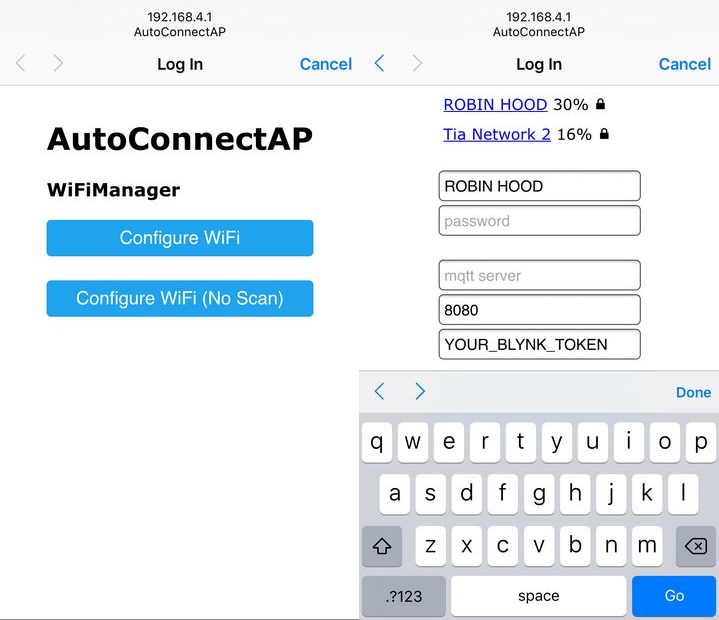
\includegraphics[scale=0.3]{images/wifi-access-point}
    \caption{Portal za odabir mreže (Izvor:~\cite{wifi-manager})}
\end{wrapfigure}

Ukoliko je dostupna mreža na koju se mikrokontroler povezao u prošlosti automatski se povezuje na nju.
U suprotnom mikrokontroler se ponaša kao pristupna točka (eng. \textit{access point}) i zahtjeva manualan odabir
bežične mreže i lozinke.
Pomoću drugog uređaja (npr.~\textit{smartphone}) potrebno je povezati se na mrežu imena \textit{ACCESS\_POINT\_NAME} s
lozinkom \textit{ACCESS\_POINT\_PASSWORD}, a potom se otvara portal kroz koji se konfigurira mreža na koju će se
mikrokontroler povezivati ubuduće.

\clearpage

\subsection{Čitanje kartice}

Nakon uspješne konfiguracije bežične veze funkcija \textit{setup} završava te započinje konstantno izvršavanje funkcije
\textit{loop}.

\begin{lstlisting}[language=C++]
void loop() {
    reader.tryReadingTheCard();
    delay(1000);
}
\end{lstlisting}

Metoda \textit{tryReadingTheCard} provjerava je li kartica prislonjena blizu čitača i pokušava pročitati UID\@.
Ovisno o uspješnosti čitanja UID-a izvršava \textit{callback-ove} definirane u \textit{setup} funkciji.
Biblioteka \textit{MFRC522} olakšava rad s NFC čitačem i instancirana je u konstruktoru klase.

\begin{lstlisting}[language=C++]
CardReader::CardReader(byte chipSelectPin, byte resetPowerDownPin) {
    reader = MFRC522(chipSelectPin, resetPowerDownPin);
}

void CardReader::tryReadingTheCard() {
    if (reader.PICC_IsNewCardPresent() == false)
        return;

    if (reader.PICC_ReadCardSerial() == false) {
        failedAttemptCallback();
        anyAttemptCallback();
        return;
    }

    Card card = Card(reader.uid);

    reader.PICC_HaltA();
    reader.PCD_StopCrypto1();

    if (card.isUidValid()) {
        successfulAttemptCallback(card);
    }
    else {
        failedAttemptCallback();
    }

    anyAttemptCallback();
}
\end{lstlisting}

Instancira se objekt \textit{Card} koji se prosljeđuje \textit{callback-u} uspješnog čitanja.
Konstruktor prima jedan argument tipa \textit{MFRC522::Uid} i pretvara ga u \textit{String}.
Klasa pruža metode za provjeru valjanosti UID-a (\textit{isUidValid}) kao i pretvaranje cijelog objekta \textit{Card} u
\textit{UID String} (\textit{toUid}).

\begin{lstlisting}[language=C++]
Card::Card(MFRC522::Uid uid) {
    UID = uidToHexString(uid);
}

String Card::uidToHexString(MFRC522::Uid uid) {
    if (uid.size == 0) return "";

    String hexString = "";

    for(unsigned short int i = 0; i < uid.size; i++) {
        const char prefix = uid.uidByte[i] < 10 ? '0' : '\0';

        String byteAsHexString = prefix + String(uid.uidByte[i], HEX);
        hexString += byteAsHexString + " ";
    }

    hexString.trim();
    hexString.toUpperCase();
    hexString.replace(' ', '-');

    return hexString;
}

bool Card::isUidValid() {
    return UID.isEmpty() == false;
}

String Card::toUid() const {
    return UID;
}
\end{lstlisting}

\subsection{Autorizacija pristupa}

Uspješnim čitanjem kartice izvršavanje programa se nastavlja u funkciji \textit{tryToAuthorizeAccess}.

\begin{lstlisting}[language=C++]
void tryToAuthorizeAccess(const Card& card) {
    Serial.println("--------------------------------------------------");
    Serial.println("Detected new card with UID: " + card.toUid());

    LED.flashGreen(1);
    delay(1000);
    LED.idle();

    if (box.isOpened()) {
        Serial.println("Box is opened, skipping...");
        LED.flashRed(1);
        return;
    }

    Serial.println("Box is closed, authorizing card with the server...");

    box.authorize(card)
       .onSuccess(grantAccess)
       .onFailure(notifyForbiddenAccess);
}
\end{lstlisting}

Jednim zelenim bljeskom LED diode korisniku se ukazuje na uspješno čitanje kartice.
Sljedeći je korak utvrditi je li kutija već otvorena (pomoću magnetskog mikroprekidača), ako je potrebno je jednim
crvenim bljeskom informirati korisnika, a izvršavanje obustaviti.

\begin{lstlisting}[language=C++]
bool Box::isOpened() const {
    return digitalRead(_statePin);
}
\end{lstlisting}

Zatvorena kutija je uvjet za slanje autorizacijskog zahtjeva na udaljeni server.

Slanje zahtjeva je izvedeno u pomoćnoj klasi \textit{POST} koja apstrahira rad s bibliotekama \textit{HTTPClient} i
\textit{WiFiClient}.
Klasa ne zna unaprijed gdje se server nalazi, koji podaci će se poslati i sl.\ već zna \textbf{kako} poslati zahtjev.

\begin{lstlisting}[language=C++]
POST::POST(): _wifiClient(), _httpClient() {
}

POST::~POST() {
    _httpClient.end();
}

POST POST::request() {
    return {};
}

POST& POST::to(const String& url) {
    _httpClient.begin(_wifiClient, url);
    _httpClient.addHeader("Content-Type", "application/x-www-form-urlencoded");

    return *this;
}

POST& POST::withPayload(const String& payload) {
    _payload = payload;

    return *this;
}

uint8_t POST::responseCode() {
    return _httpClient.POST(_payload);
}
\end{lstlisting}

Metode \textit{POST} klase su iskorištene u metodi \textit{BoxAuthorizer::authorize}.
Ova metoda ne zna kako poslati zahtjev ali zna \textbf{gdje} i \textbf{koje} podatke treba poslati.
Prosljeđuje se URL adresa udaljenog servera i UID\@.
Ukoliko je HTTP kod odgovara jednak 200 autorizacija je uspješna.

\begin{lstlisting}[language=C++]
BoxAuthorizer::Result BoxAuthorizer::authorize(const String &uid) {
    return POST::request()
                 .to("http://144.126.244.106/api/box/authorize")
                 .withPayload("uid=" + uid)
                 .responseCode() == 200
                                  ? authorizationSucceeded()
                                  : authorizationFailed();
}
\end{lstlisting}
